\documentclass{standalone}
\usepackage[T1]{fontenc}
\usepackage[utf8]{inputenc}
\usepackage[usenames,dvipsnames]{xcolor}
\usepackage{tikz}
\usetikzlibrary{plotmarks}
\usetikzlibrary{shapes,snakes,arrows}
\begin{document}
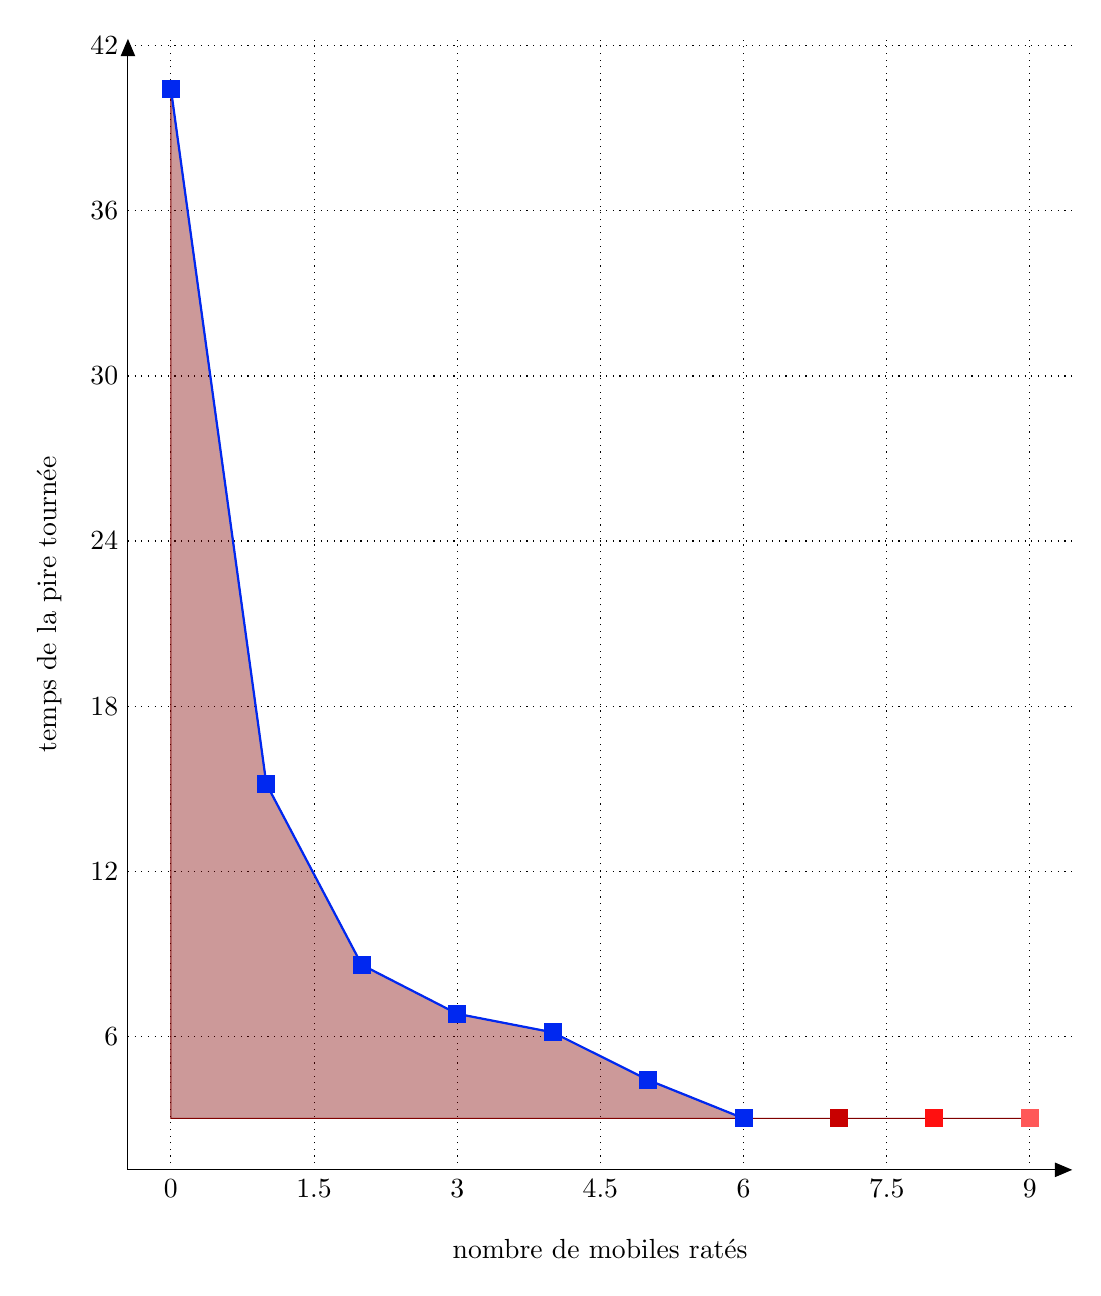
\begin{tikzpicture}[xscale=1.21212,yscale=0.349404]
\draw[xstep=1.5,ystep=6,thin,dotted,color=Black] (-0.45,1.145) grid (9.44363,42.2518);
\begin{scope}
  \clip (-0.45,1.145) rectangle (9.44363,42.2518);
  \definecolor{hvColor}{RGB}{128,0,0}
  \draw[color=hvColor, fill=hvColor, fill opacity=0.4] (0,3.0158) -- (0,40.4317) -- (1,15.1743) -- (2,8.59572) -- (3,6.81689) -- (4,6.14226) -- (5,4.41054) -- (6,3.0158) -| (9,3.0158) -- cycle;
  \definecolor{pLineColor}{RGB}{128,0,0}
  \definecolor{pPointColor}{RGB}{0,40,240}
  \draw[thick,color=pPointColor] (0,40.4317) node[draw,color=pPointColor,fill=pPointColor, inner sep = 0pt, minimum size=2mm] {} -- (1,15.1743) node[draw,color=pPointColor,fill=pPointColor, inner sep = 0pt, minimum size=2mm] {} -- (2,8.59572) node[draw,color=pPointColor,fill=pPointColor, inner sep = 0pt, minimum size=2mm] {} -- (3,6.81689) node[draw,color=pPointColor,fill=pPointColor, inner sep = 0pt, minimum size=2mm] {} -- (4,6.14226) node[draw,color=pPointColor,fill=pPointColor, inner sep = 0pt, minimum size=2mm] {} -- (5,4.41054) node[draw,color=pPointColor,fill=pPointColor, inner sep = 0pt, minimum size=2mm] {} -- (6,3.0158) node[draw,color=pPointColor,fill=pPointColor, inner sep = 0pt, minimum size=2mm] {};
  \definecolor{pLineColor}{RGB}{200,0,0}
  \definecolor{pPointColor}{RGB}{200,0,0}
  \draw[thick,color=pPointColor] (7,3.0158) node[draw,color=pPointColor,fill=pPointColor, inner sep = 0pt, minimum size=2mm] {};
  \definecolor{pLineColor}{RGB}{255,16,16}
  \definecolor{pPointColor}{RGB}{255,16,16}
  \draw[thick,color=pPointColor] (8,3.0158) node[draw,color=pPointColor,fill=pPointColor, inner sep = 0pt, minimum size=2mm] {};
  \definecolor{pLineColor}{RGB}{255,88,88}
  \definecolor{pPointColor}{RGB}{255,88,88}
  \draw[thick,color=pPointColor] (9,3.0158) node[draw,color=pPointColor,fill=pPointColor, inner sep = 0pt, minimum size=2mm] {};
\end{scope}
\draw[->,>=triangle 45] (-0.45,1.145) -- coordinate (x axis mid) (9.44363,1.145);
\node[below=1cm,anchor=center] at (x axis mid) {nombre de mobiles ratés};
\foreach \x in {0,1.5,3,4.5,6,7.5,9}
  \draw (\x,1.145) -- (\x,1.145) node[anchor=north] {\x};
\draw[->,>=triangle 45] (-0.45,1.145) -- coordinate (y axis mid) (-0.45,42.2518);
\node[left=1cm,rotate=90,anchor=center] at (y axis mid) {temps de la pire tournée};
\foreach \y in {6,12,18,24,30,36,42}
  \draw (-0.45,\y) -- (-0.45,\y) node[anchor=east] {\y};
\end{tikzpicture}
\end{document}
